
\usetikzlibrary{shapes.geometric,calc}

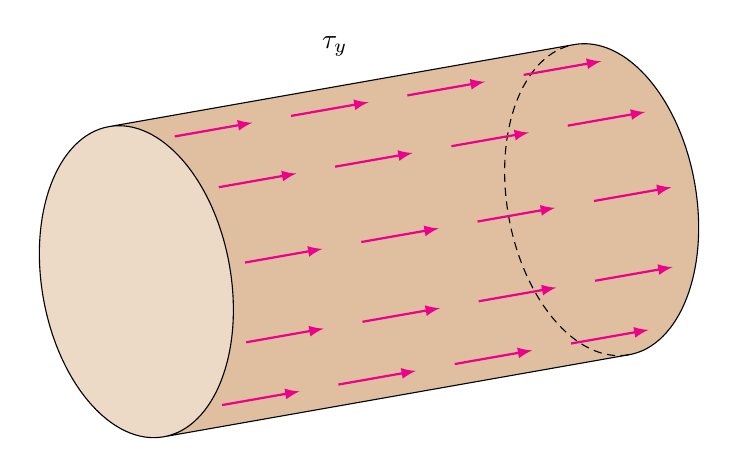
\begin{tikzpicture}[rotate = 100]

%\node [cylinder, draw,rotate=190, minimum height=3cm, minimum width=1.3cm,shape aspect=3,cylinder uses custom fill,cylinder body fill=brown!60,cylinder end fill=brown!25] (c) {};
    
%\node[cylinder,draw=black,thick,aspect=0.7,minimum height=1.7cm,minimum width=1.5cm,shape border rotate=90,cylinder uses custom fill, cylinder body fill=red!30,cylinder end fill=red!10] (A) {A};
  
  
%\fill[top color=brown!50!black,bottom color=brown!10,middle color=brown,shading=axis,opacity=0.25] (0,0) circle (2cm and 0.5cm);
%\fill[left color=brown!50!black,right color=brown!50!black,middle color=brown!50,shading=axis,opacity=0.25] (2,0) -- (2,6) arc (360:180:2cm and 0.5cm) -- (-2,0) arc (180:360:2cm and 0.5cm);
%\fill[top color=brown!90!,bottom color=brown!2,middle color=brown!30,shading=axis,opacity=0.25] (0,6) circle (2cm and 0.5cm);



\def \R {2};
\def \r {1.2}

\fill[color=brown!25,opacity=1] (0,0) circle (\R cm and \r cm);
\fill[color=brown!50,opacity=1] (\R,0) -- (\R,6) arc (360:180:\R cm and \r cm) -- (-\R,0) arc (180:360:\R cm and \r cm);
\fill[color=brown!30,opacity=1] (0,6) circle (\R cm and \r cm);

\draw (-\R,6) -- (-\R,0) arc (180:360:\R cm and \r cm) -- (\R,6) ++ (-\R,0) circle (\R cm and \r cm);
\draw[densely dashed] (-\R,0) arc (180:0:\R cm and \r cm);

\node at (\R+0.5,3)  {$\tau_{\text{y}}$}; 

\foreach \y in {-1.2,0.3,...,4} {
	 \foreach \x in {30,60,...,150} {
                \draw[latex-,magenta,thick] ({cos(\x)*\R}, {\y+1.5-\r*sin(\x)})  -- ({\R*cos(\x)}, {\y+1.5+1-\r*sin(\x)});
        }
}

\end{tikzpicture}